\documentclass[aps,prl,twocolumn,showpacs,amsmath,amssymb]{revtex4-1}
%\documentclass[aps,prl,twocolumn,showpacs,preprintnumbers,amsmath,amssymb,citeautoscript]{revtex4-1}
%\documentclass[prl,showpacs,amssymb,amsmath,twocolumn]{revtex4-1}
%%%%%%%%%%%%
\usepackage{bookmath} % definitions and shortcuts
%%%%%%%%%%%%
\usepackage{graphicx}
\usepackage{amsmath}
\usepackage{color}
\newcommand{\blue}{\textcolor{blue}}
\newcommand{\red}{\textcolor{red}}
\newcommand{\cecoin}{CeCoIn$_5$} 
\def\opp#1{{\overline{ #1}}}

\bibliographystyle{apsrev4-1}
%~~~~~~~~~~~~~~~~~~~~~~~~~~~~~~~~~~~~~~~~~~~~~~~~~~~~~~~~~~~~~~~~~~~~~~~~~~~~~~~%
\begin{document}
%~~~~~~~~~~~~~~~~~~~~~~~~~~~~~~~~~~~~~~~~~~~~~~~~~~~~~~~~~~~~~~~~~~~~~~~~~~~~~~~%
\title{Electronic Spin Susceptibility in Superconductor-Normal Metal Interfaces}

\author{Benjamin~M.~Rosemeyer}
\author{Anton~B.~Vorontsov}

\affiliation{Department of Physics, Montana State University, Montana 59717, USA}

\date{\today}

\begin{abstract}
%
We calculate the wave-vector dependent electronic spin susceptibility 
$\chi_{\alpha\beta}(\vq, \vH_0, \vR)$ 
around a Superconductor-Normal metal interface with and without a uniform magnetic field $\vH_0$ at zero temperature. 
We consider the 2D cylindrical Fermi surface of free electrons ($\xi_\vk = \frac{\vk^2}{2m^*}-\epsilon_F$) on both sides of the interface.
For the superconductor we consider both S and D-wave order parameters.
We identify several features such as the tendency for enhanced susceptibility for wave vectors $\vq$ which correspond to those defined by the distance $\vR$ from the interface and it's steepness.
%
\end{abstract} 

\pacs{74.20.Rp,74.25.Ha,74.70.Tx} 

\maketitle


%~~~~~~~~~~~~~~~~~~~~~~~~~~~~~~~~~~~~~
\section*{Introduction}
%~~~~~~~~~~~~~~~~~~~~~~~~~~~~~~~~~~~~~
%

%~~~~~~~~~~~~~~~~~~~~~~~~~~~~~~~~~~~~~
\section*{Equations}
%~~~~~~~~~~~~~~~~~~~~~~~~~~~~~~~~~~~~~
%
Our model is a position dependent, mean-field SC Hamiltonian with 2D cylindrical FS,
and electrons interacting with uniform magnetic field $\vH_0$ through Zeeman term: 
$ \cH = \cH_{0} + V  $
\be\label{eq:modelH} 
\begin{split}
\cH_{0}(\vr) = \sum_{\vk \mu} \xi_\vk c^\dag_{\vk \mu} c_{\vk \mu} 
+ \sum_\vk \left( \Delta_\vk(\vr) c_{\vk \uparrow}^\dag c_{-\vk \downarrow}^\dag + h.c. \right) 
\\
+ \mu_\sm{B} \sum_{\vk \mu \nu} c^\dag_{\vk\mu} \, \vsigma_{\mu\nu} \vH_0 \, c_{\vk\nu}  
\end{split}
\ee
and for linear response we include a $\vq$-dependent perturbation 
of the magnetic field $\delta\vH(\vR) = \delta\vH_\vq e^{i\vq\cdot\vR}$, 
$V = \mu_\sm{B} \sum_{\vk \mu \nu} c^\dag_{\vk+\vq \mu}  \, \vsigma_{\mu\nu} \delta\vH_\vq \, c_{\vk \nu}  $, where $\mu_\sm{B}$ is the magnetic moment of electron.
The electronic dispersion in the normal state is $\xi_{\vk}=\frac{\vk^2}{2m^*}-\epsilon_F$.  
The resulting magnetization has uniform part and $\vq$-dependent perturbation:
\be
M_\alpha(\vR) = M_{0\alpha}(\vR,\vH_0) + 
\chi_{\alpha\beta} (\vR,\vq) \delta H_\beta e^{i\vq \cdot \vR}
\ee
with 
$\vM_0(\vR,t) = \mu_\sm{B} \langle \vS(\vR,t) \rangle_0 $, 
and susceptibility is a two particle correlation function~\cite{mahan}: 
\be
\label{eq:susdef}
\chi_{\alpha\beta}(\vx,\vx', t)= \frac{i \mu_\sm{B}^2}{\hbar} 
\langle [ S_\alpha(\vx,t), S_\beta(\vx',0) ] \theta(t) \rangle_0 
\ee

where 
$\vS(\vx,t) = \sum_{\mu \nu} \psi^\dag_\mu(\vx,t) \, \vsigma_{\mu\nu} \, \psi_{\nu}(\vx,t)$,  
$\psi_{\nu}(\vx,t) = \sum_\vk c_{\vk \nu} (t) \varphi_{\vk\nu}(\vx)$, 
$c_{\vk \nu} (t) = e^{i\cH_0 t} c_{\vk \mu} e ^{-i \cH_0 t}$, $\varphi_{\vk\nu} = e^{i\vk_{\nu}\cdot\vx}$; 
subscript $0$ indicates the average over ensemble (\ref{eq:modelH}).


\begin{widetext}
\begin{align*}
&\chi(\vr_x,q_y,\vR=0) = \frac{\mu_B^2}{\hbar}\sum\limits_{\vk\vp_x\mu}   \\
&\bigg[(u_{\vk1} \, v_{\vk2} \, v_{\vp1} \, u_{\vp2}-u_{\vk1} \, u_{\vk2} \, v_{\vp1} \, v_{\vp2})e^{i(-\vk1_x\vr_x/2-\vk2_x\vr_x/2-\vp1_x\vr_x/2-\vp2_x\vr_x/2)}\bigg|_{-\vk1_y-\vp1_y-q_y=0}\\
& + (u_{\vk2} \, v_{\vk1} \, v_{\vp2} \, u_{\vp1}- v_{\vk1} \, v_{\vk2} \,u_{\vp1} \, u_{\vp2} )e^{i(\vk1_x\vr_x/2+\vk2_x\vr_x/2+\vp1_x\vr_x/2+\vp2_x\vr_x/2)}\bigg|_{\vk1_y+\vp1_y-q_y=0}\bigg] \frac{1-f_{-\vp1}-f_{\vk1}}{\omega_{\vk1} +\omega_{-\vp1}} \\
\\
&+\bigg[(u_{\vk1} \, u_{\vk2} \, u_{\vp1} \, u_{\vp2}+ u_{\vk1} \, v_{\vk2} \, v_{\vp2} \, u_{\vp1})e^{i(-\vk1_x\vr_x/2-\vk2_x\vr_x/2+\vp1_x\vr_x/2+\vp2_x\vr_x/2)}\bigg|_{-\vk1_y+\vp1_y-q_y=0} \\
& + (v_{\vk1} \, v_{\vk2} \,v_{\vp1} \, v_{\vp2} +u_{\vk2} \, v_{\vk1} \,v_{\vp1} \, u_{\vp2})e^{i(\vk1_x\vr_x/2+\vk2_x\vr_x/2-\vp1_x\vr_x/2-\vp2_x\vr_x/2)}\bigg|_{\vk1_y-\vp1_y-q_y=0} \bigg]\frac{f_{\vk1} - f_{\vp1}}{\omega_{\vk1} - \omega_{\vp1}}
\end{align*}
\end{widetext}

To find the Fourier Transform wrt the x coordinate we can use a fast fourier transform from the spacial domain $x\in[-L:L]$ to momentum space $q_x\in[-n\pi:n\pi]$ using $2N+1$ points ($N=nL$):
\be
\chi(\vq) = \sum\limits_{i=1}^{2*N+1}e^{-iq_x\vr_x(i)}\chi(\vr_x(i),q_y,\vR=0)
\ee

% NOTE: currently I am only looking at the real part of $\chi(\vr,\vR=0)$, so the exponentials turn into cosines and I have $\pm$ symmetry for $x$ and my FT looks like
% 
% \be
% \chi(\vq) = \sum\limits_{i=1}^{N+1}\cos(q_x\vr_x(i))\chi(\vr_x(i),q_y,\vR=0)
% \ee
% 
\begin{widetext}
%~~~~~~~~~~~~~~~~~~~~~~~~~~~~~~~~~~~~~
\section*{Results}
%~~~~~~~~~~~~~~~~~~~~~~~~~~~~~~~~~~~~~
%

Below are surface plots for the 2D Normalized susceptibility for various conditions.

The $q/k_f$ axis is the in the $\hat{x}$, and the $xk_f$ axis indicates the distance from the domain wall which is at $xk_f = 0$.

For all the plots, $\Delta = 0.05\epsilon_f$, and $T=0$

%%%%%%%%%%%%%%%%%%%%%%%%%%%%%%%%%%%%%%%%%%%%%%%%%%%%%%%%%%%%%%%%%%%%%%%%%%%%%%%%%
\begin{figure}
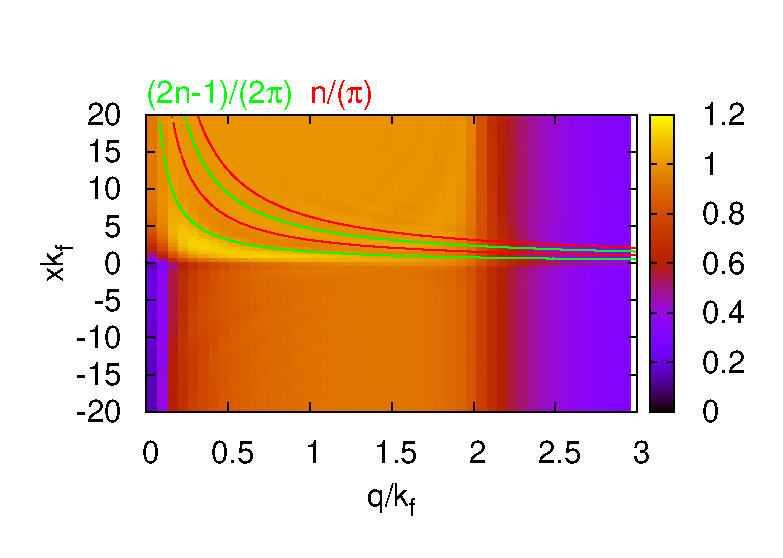
\includegraphics[width=0.7\linewidth]{surface_perp_s_noF.eps}
\caption{ 
	\label{fig:qq} S wave, No Field
} 
\end{figure}
%%%%%%%%%%%%%%%%%%%%%%%%%%%%%%%%%%%%%%%%%%%%%%%%%%%%%%%%%%%%%%%%%%%%%%%%%%%%%%%%%
%%%%%%%%%%%%%%%%%%%%%%%%%%%%%%%%%%%%%%%%%%%%%%%%%%%%%%%%%%%%%%%%%%%%%%%%%%%%%%%%%
\begin{figure}
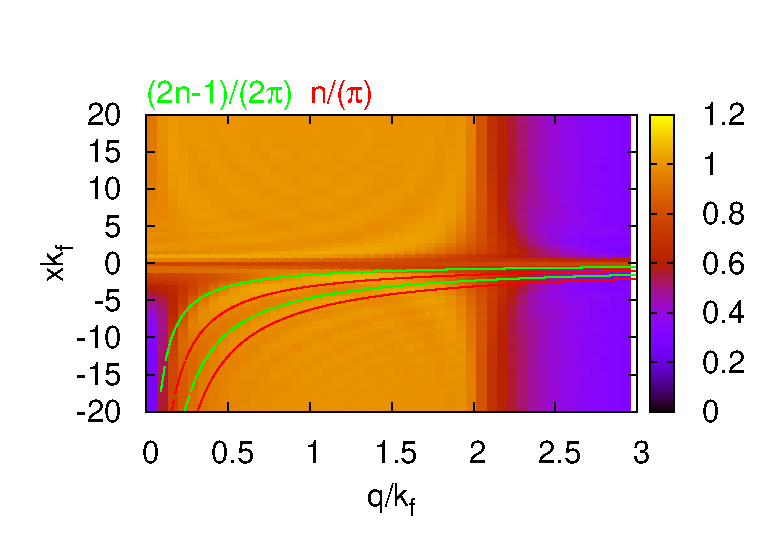
\includegraphics[width=0.7\linewidth]{surface_perp_d_noF.eps}
\caption{ 
	\label{fig:qq} D wave, No Field
} 
\end{figure}
%%%%%%%%%%%%%%%%%%%%%%%%%%%%%%%%%%%%%%%%%%%%%%%%%%%%%%%%%%%%%%%%%%%%%%%%%%%%%%%%%
%%%%%%%%%%%%%%%%%%%%%%%%%%%%%%%%%%%%%%%%%%%%%%%%%%%%%%%%%%%%%%%%%%%%%%%%%%%%%%%%%
\begin{figure}
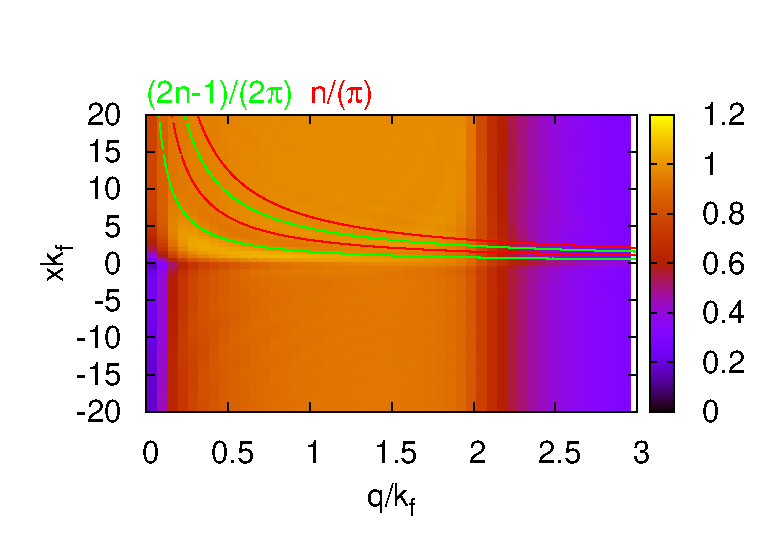
\includegraphics[width=0.7\linewidth]{surface_perp_s_F.eps}
\caption{ 
	\label{fig:qq} S wave, $\perp$ Field ($\mu_B H=0.6\Delta_0$)
} 
\end{figure}
%%%%%%%%%%%%%%%%%%%%%%%%%%%%%%%%%%%%%%%%%%%%%%%%%%%%%%%%%%%%%%%%%%%%%%%%%%%%%%%%%
%%%%%%%%%%%%%%%%%%%%%%%%%%%%%%%%%%%%%%%%%%%%%%%%%%%%%%%%%%%%%%%%%%%%%%%%%%%%%%%%%
\begin{figure}
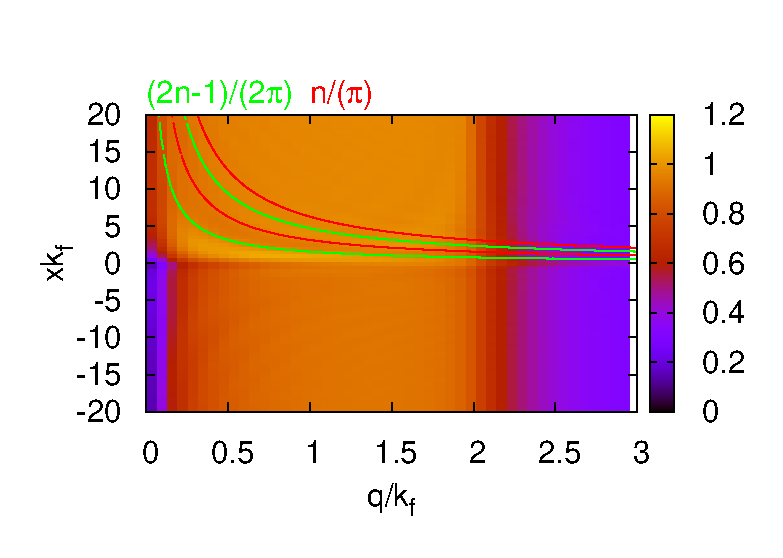
\includegraphics[width=0.7\linewidth]{surface_para_s_F.eps}
\caption{ 
	\label{fig:qq} S wave, $\parallel$ Field ($\mu_B H=0.6\Delta_0$)
} 
\end{figure}
%%%%%%%%%%%%%%%%%%%%%%%%%%%%%%%%%%%%%%%%%%%%%%%%%%%%%%%%%%%%%%%%%%%%%%%%%%%%%%%%%
%%%%%%%%%%%%%%%%%%%%%%%%%%%%%%%%%%%%%%%%%%%%%%%%%%%%%%%%%%%%%%%%%%%%%%%%%%%%%%%%%
\begin{figure}
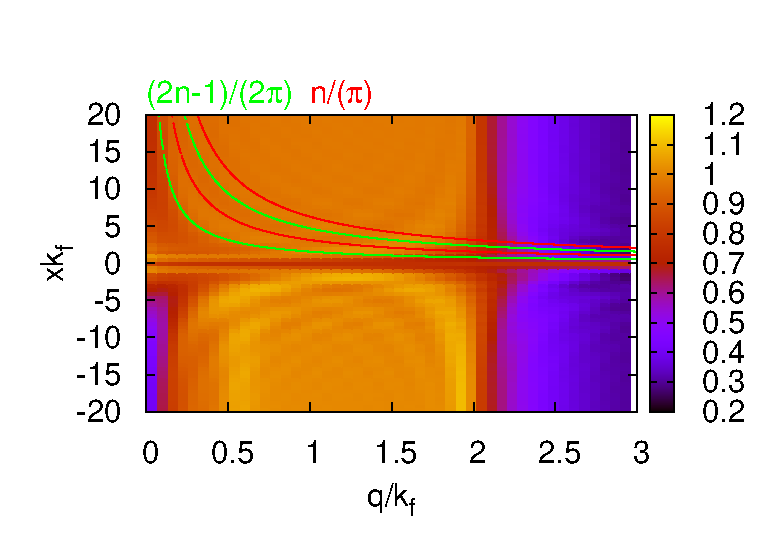
\includegraphics[width=0.7\linewidth]{surface_perp_d_F.eps}
\caption{ 
	\label{fig:qq} D wave, $\perp$ Field ($\mu_B H=0.6\Delta_0$)
} 
\end{figure}
%%%%%%%%%%%%%%%%%%%%%%%%%%%%%%%%%%%%%%%%%%%%%%%%%%%%%%%%%%%%%%%%%%%%%%%%%%%%%%%%%
%%%%%%%%%%%%%%%%%%%%%%%%%%%%%%%%%%%%%%%%%%%%%%%%%%%%%%%%%%%%%%%%%%%%%%%%%%%%%%%%%
\begin{figure}
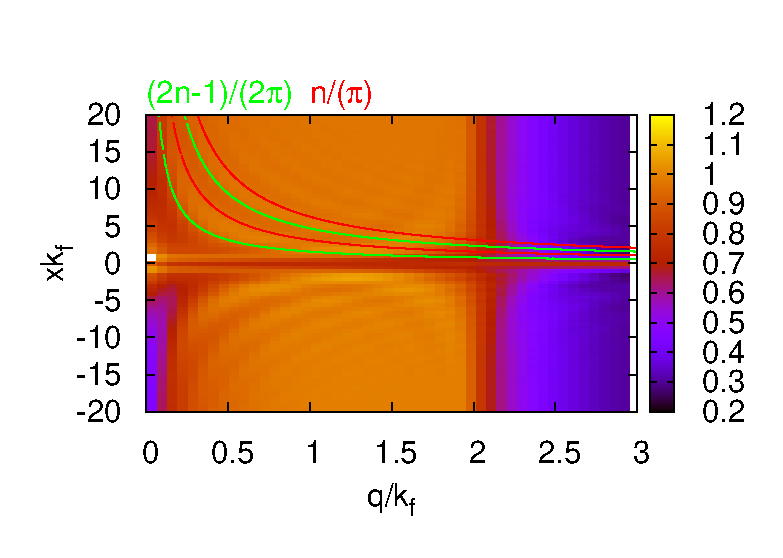
\includegraphics[width=0.7\linewidth]{surface_para_d_F.eps}
\caption{ 
	\label{fig:qq} D wave, $\parallel$ Field ($\mu_B H=0.6\Delta_0$)
} 
\end{figure}
%%%%%%%%%%%%%%%%%%%%%%%%%%%%%%%%%%%%%%%%%%%%%%%%%%%%%%%%%%%%%%%%%%%%%%%%%%%%%%%%%
%%%%%%%%%%%%%%%%%%%%%%%%%%%%%%%%%%%%%%%%%%%%%%%%%%%%%%%%%%%%%%%%%%%%%%%%%%%%%%%%%
\begin{figure}
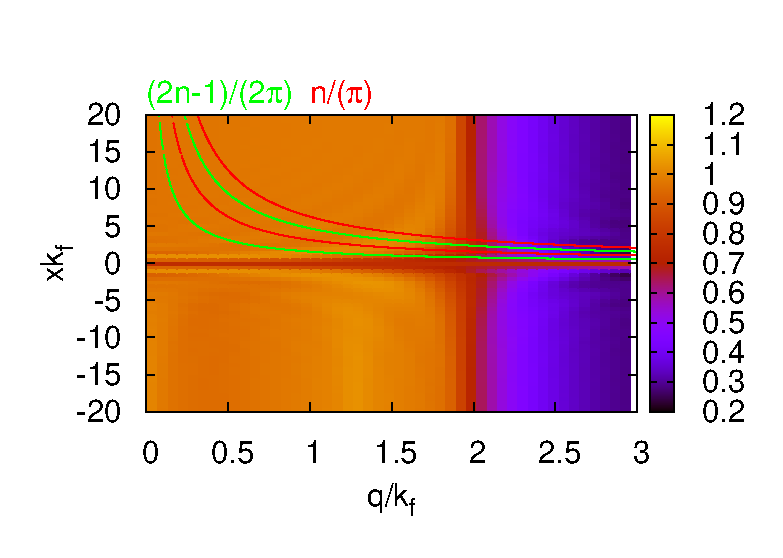
\includegraphics[width=0.7\linewidth]{surface_perp_d_Fqs.eps}
\caption{ 
	\label{fig:qq} D wave, $\perp$ Field ($\mu_B H=0.6\Delta_0$), with $q_y = 0.63$
} 
\end{figure}
%%%%%%%%%%%%%%%%%%%%%%%%%%%%%%%%%%%%%%%%%%%%%%%%%%%%%%%%%%%%%%%%%%%%%%%%%%%%%%%%%
%%%%%%%%%%%%%%%%%%%%%%%%%%%%%%%%%%%%%%%%%%%%%%%%%%%%%%%%%%%%%%%%%%%%%%%%%%%%%%%%%
\begin{figure}
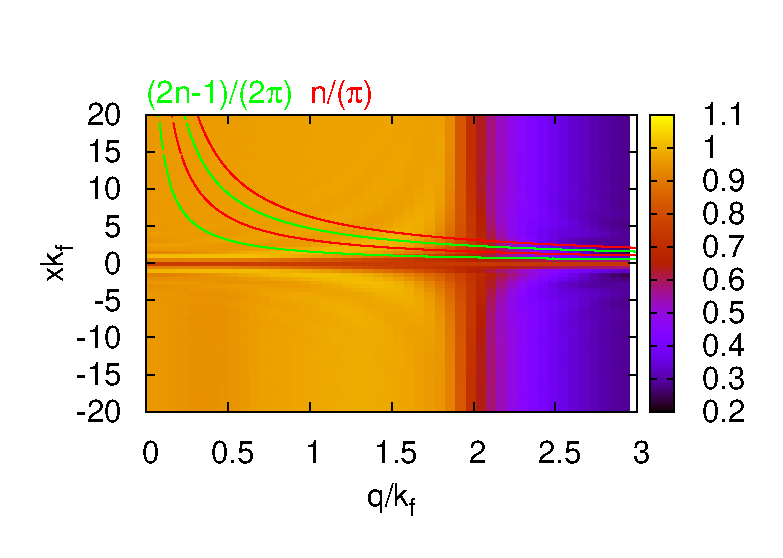
\includegraphics[width=0.7\linewidth]{surface_para_d_Fqs.eps}
\caption{ 
	\label{fig:qq} D wave, $\parallel$ Field ($\mu_B H=0.6\Delta_0$), with $q_y = 0.63$
} 
\end{figure}
%%%%%%%%%%%%%%%%%%%%%%%%%%%%%%%%%%%%%%%%%%%%%%%%%%%%%%%%%%%%%%%%%%%%%%%%%%%%%%%%%
%%%%%%%%%%%%%%%%%%%%%%%%%%%%%%%%%%%%%%%%%%%%%%%%%%%%%%%%%%%%%%%%%%%%%%%%%%%%%%%%%
\begin{figure}
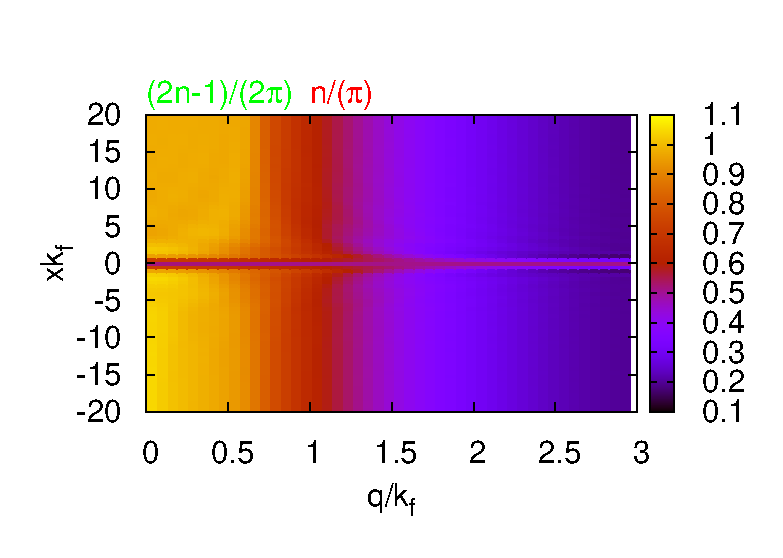
\includegraphics[width=0.7\linewidth]{surface_perp_d_Fql.eps}
\caption{ 
	\label{fig:qq} D wave, $\perp$ Field ($\mu_B H=0.6\Delta_0$), with $q_y = 1.89$
} 
\end{figure}
%%%%%%%%%%%%%%%%%%%%%%%%%%%%%%%%%%%%%%%%%%%%%%%%%%%%%%%%%%%%%%%%%%%%%%%%%%%%%%%%%
%%%%%%%%%%%%%%%%%%%%%%%%%%%%%%%%%%%%%%%%%%%%%%%%%%%%%%%%%%%%%%%%%%%%%%%%%%%%%%%%%
\begin{figure}
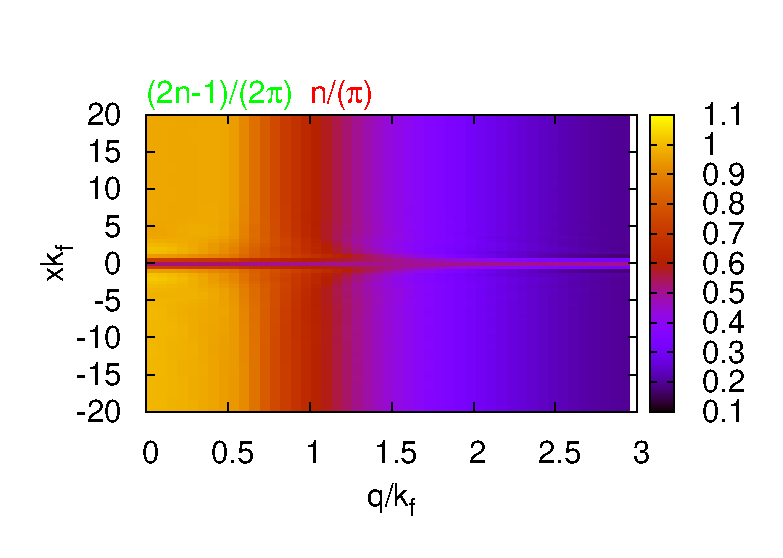
\includegraphics[width=0.7\linewidth]{surface_para_d_Fql.eps}
\caption{ 
	\label{fig:qq} D wave, $\parallel$ Field ($\mu_B H=0.6\Delta_0$), with $q_y = 1.89$
} 
\end{figure}
%%%%%%%%%%%%%%%%%%%%%%%%%%%%%%%%%%%%%%%%%%%%%%%%%%%%%%%%%%%%%%%%%%%%%%%%%%%%%%%%%
\end{widetext}
 %~~~~~~~~~~~~~~~~~~~~~~~~~~~~~~~~~~~~~~~~~~~~~~~~~~~~~~~~~~~~~~~~~~~~~~~~~~~~~~~
  %~~~~~~~~~~~~~~~~~~~~~~~~~~~~~~~~~~~~~~~~~~~~~~~~~~~~~~~~~~~~~~~~~~~~~~~~~~~~~~~
   %~~~~~~~~~~~~~~~~~~~~~~~~~~~~~~~~~~~~~~~~~~~~~~~~~~~~~~~~~~~~~~~~~~~~~~~~~~~~~~~
    %~~~~~~~~~~~~~~~~~~~~~~~~~~~~~~~~~~~~~~~~~~~~~~~~~~~~~~~~~~~~~~~~~~~~~~~~~~~~~~~
     %~~~~~~~~~~~~~~~~~~~~~~~~~~~~~~~~~~~~~~~~~~~~~~~~~~~~~~~~~~~~~~~~~~~~~~~~~~~~~~~
      %~~~~~~~~~~~~~~~~~~~~~~~~~~~~~~~~~~~~~~~~~~~~~~~~~~~~~~~~~~~~~~~~~~~~~~~~~~~~~~~

\bibliography{mybib}

%~~~~~~~~~~~~~~~~~~~~~~~~~~~~~~~~~~~~~~~~~~~~~~~~~~~~~~~~~~~~~~~~~~~~~~~~~~~~~~~%
\end{document}
%~~~~~~~~~~~~~~~~~~~~~~~~~~~~~~~~~~~~~~~~~~~~~~~~~~~~~~~~~~~~~~~~~~~~~~~~~~~~~~~%
